\section{Visualisation of Lagrangian Coherent Structures}

Motivation: Vector field topology does not well describe the topology of a "strongly" time-dependent vector field. 
\begin{description}
\item Separatrices are defined in terms of streamlines, not pathlines.
\item Critical points of a saddle types are not the places where flow separation happens.
\end{description}

\subsection{The Finite-Time Lyapunov Exponent}
The FTLE describes the amount of separation (stretching) after a finite advection time $T$.

Principle:
\begin{figure}[H]
    \centering
    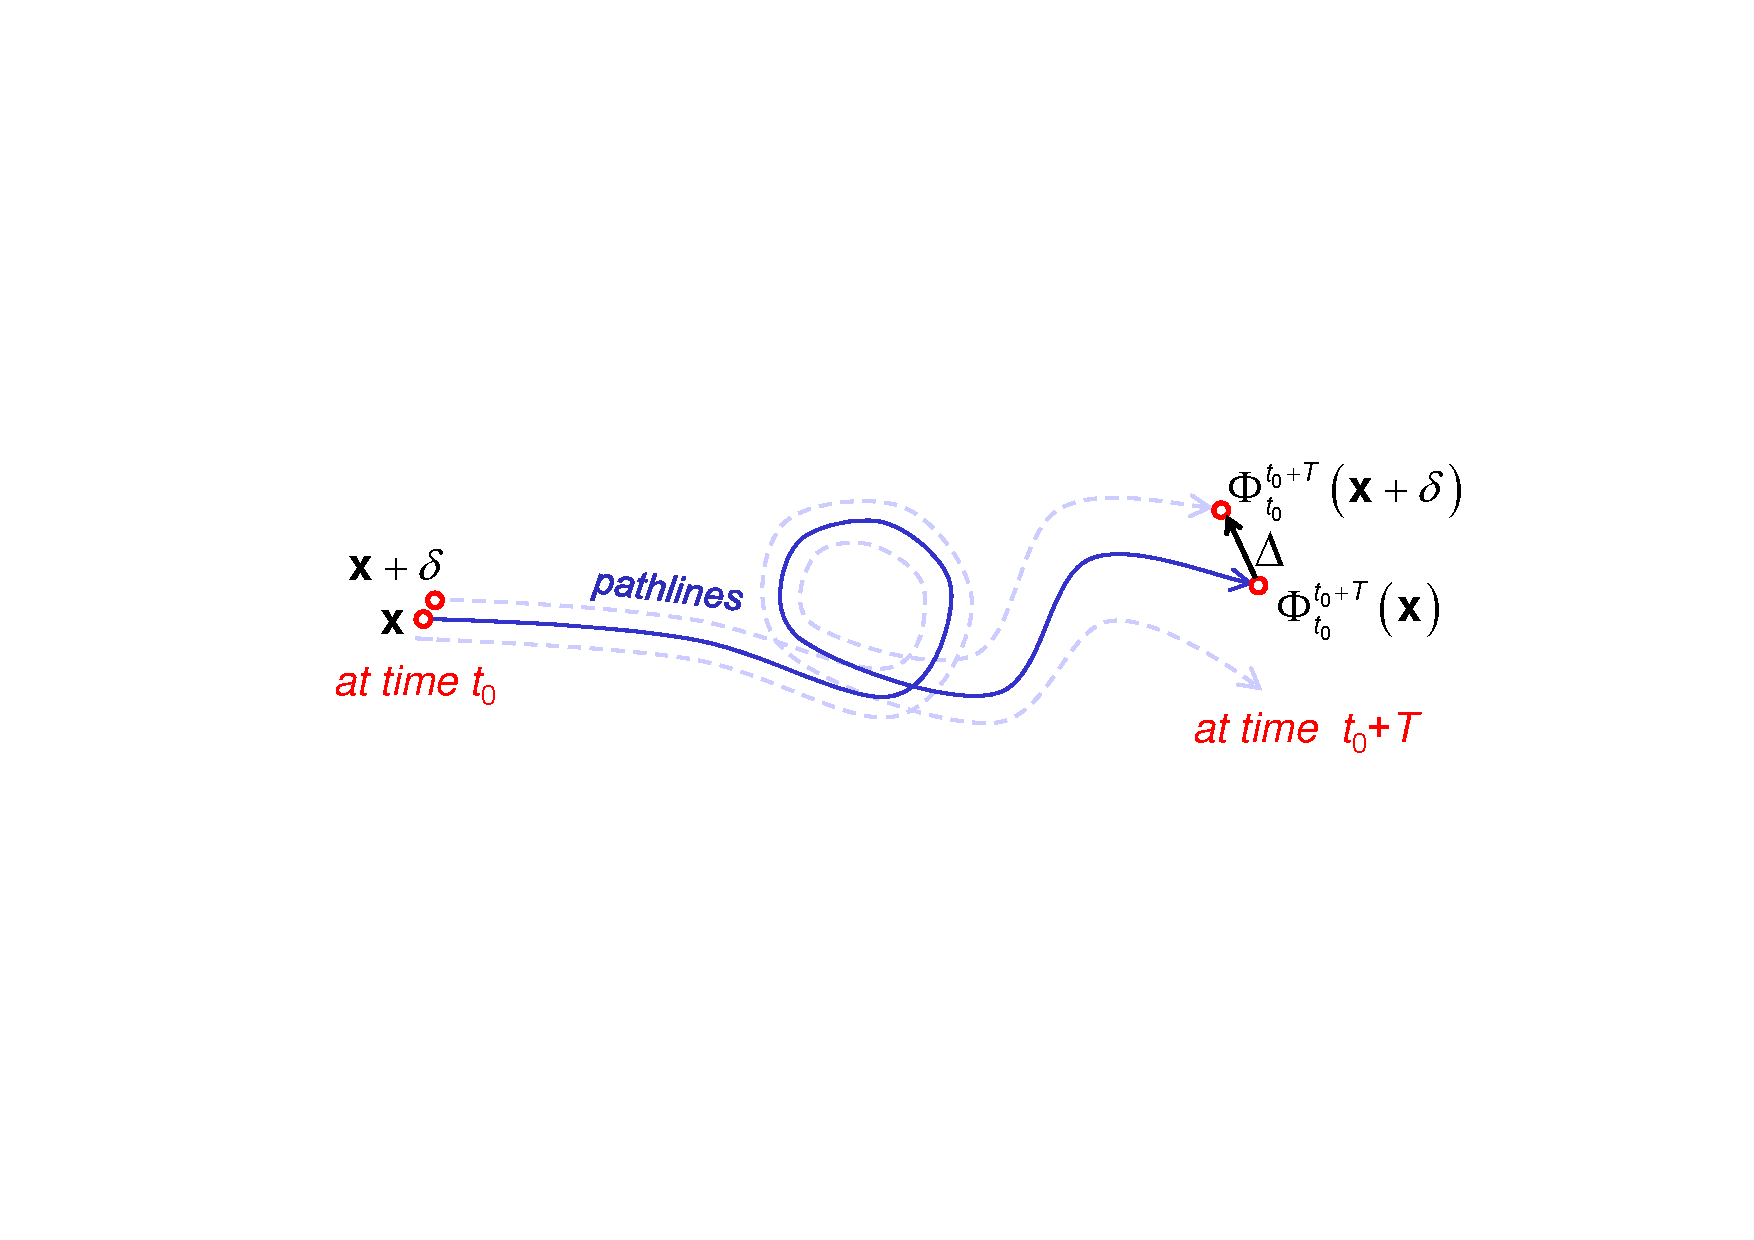
\includegraphics[width=0.7\textwidth]{img/09_ftle}
\end{figure}
Definition:
\begin{align*}
    \text{FTLE}(x,t_0,T) = \lim_{\delta\rightarrow 0} \max_{\text{direction of }\delta} {1\over |T|} \log\left( {\norm{\Delta}\over \norm{\delta}}\right)  = {1\over |T|} \log\left(
        \sqrt{\lambda_{\max} (F^*F)}
    \right)
\end{align*}
with $F=\nabla \Phi_{t_0}^{t_0+T} (x)$ and $F^* F$ being the Cauchy-Green deformation tensor.

\paragraph{Application}
\begin{enumerate}
    \item Compute the flow map: 
        \begin{align*}
         x&\mapsto \Phi_t^{t+T} (x) &\text{(for fixed times $t$, $t+T$)}
        \end{align*}
        \begin{figure}[H]
            \centering
            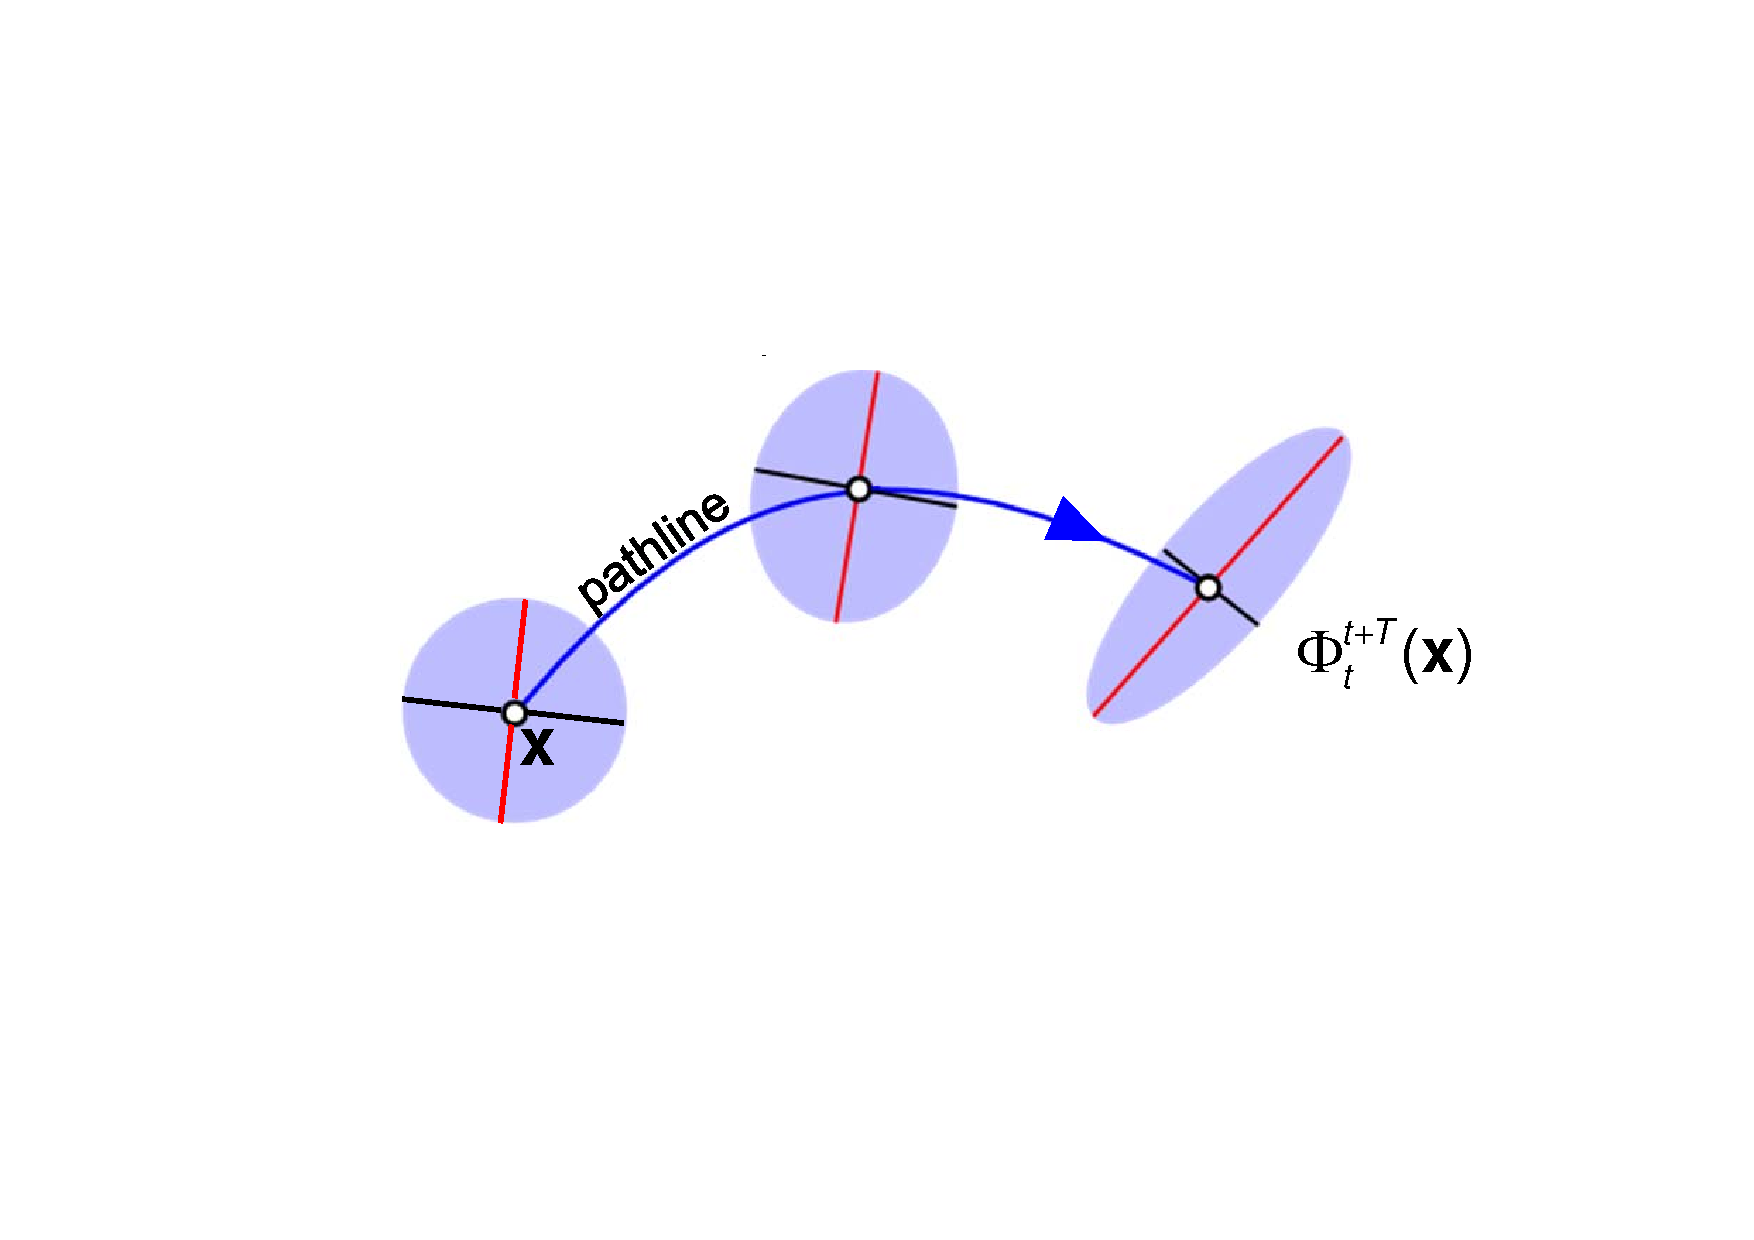
\includegraphics[width=0.6\textwidth]{img/09_lcs_application}
        \end{figure}

    \item Compute Cauchy-Green tensor:
        \begin{align*}
            C &= F^*F\\
            F &= \nabla \Phi_t^{t_T} (x)
        \end{align*}
    \item FTLE:
        \begin{align*}
             \sigma = {1\over |T|} \log \sqrt{\lambda_1(C)}
        \end{align*}
\end{enumerate}
\subsection{Separatrices}
Separatrix: A streamline converging to a saddle point (interesting because it acts as a flow barrier). 
\begin{itemize}
    \item Convergence in positive time: \emph{Attracting separatrix}.
    \item Convergence in negative time: \emph{Repelling separatrix}.
\end{itemize}

\subsubsection{LCS in 3D} 
Visualise using \emph{direct volume rendering}. Use a transfer function which maps high FTLE values to high opacity: Approximates ridges.

LCSs have replaced VFT in feature-based visualisation of \emph{unsteady} flow. Two approaches are commonly used:
\begin{itemize}
    \item Geometric extraction of ridges
    \item Visualisation focusing on high FTLE values:
        \begin{itemize}
            \item Isosurfaces
            \item DVR
        \end{itemize}
\end{itemize}
Advantages of \emph{geometric} ridges:
\begin{itemize}
    \item Follows Haller's definition more strictly.
    \item Allows for quantitative checking of cross-flux.
\end{itemize}

\subsection{Computation of FTLE Ridges}
Efficient computation of height ridges (of a scalar field $s(x)$ in $n$-space):
\begin{itemize}
\item Compute derived fields $g=\nabla s$ and $H=\nabla g$
\item For ridges of \emph{dimension 1} use the \emph{Parallel Vectors method}:
    \begin{itemize}
        \item Find the places where $g$ and $Hg$ are parallel vectors.
        \item Compute the eigenvalues of $H$, test if those in the directions of $\perp g$ are all negative and less than the one in direction $g$
    \end{itemize}
\item For ridges of \emph{co-dimension 1} (i.e. of dimension $n-1$) use \emph{Marching Ridges} method (Furst et al. 2001):
    \begin{itemize}
        \item Compute eigenvalues of $H$: $\lambda_1 \leq \ldots \leq \lambda_n$
        \item $\varepsilon_1$: Eigenvector for $\lambda_1$ ($\varepsilon_1 \perp $ ridge)
        \item Solve for $\varepsilon_1 \cdot g=0$ (single scalar equation!)
    \end{itemize}

    Problem: $\varepsilon_1$ is not a vector field (ambiguous directions). Marching Ridges does the following per cell:
    
    \begin{itemize}
        \item Orient $\varepsilon_1$ at nodes of the cell by PCA.
        \item Evaluate $\varepsilon_1\cdot g$ at node
        \item Interpolate zero crossings on edges
        \item Use zero crossings with $\lambda_1 < 0$
        \item Generate triangles for \emph{Marching Cubes} case:
            \begin{figure}[H]
                \centering
                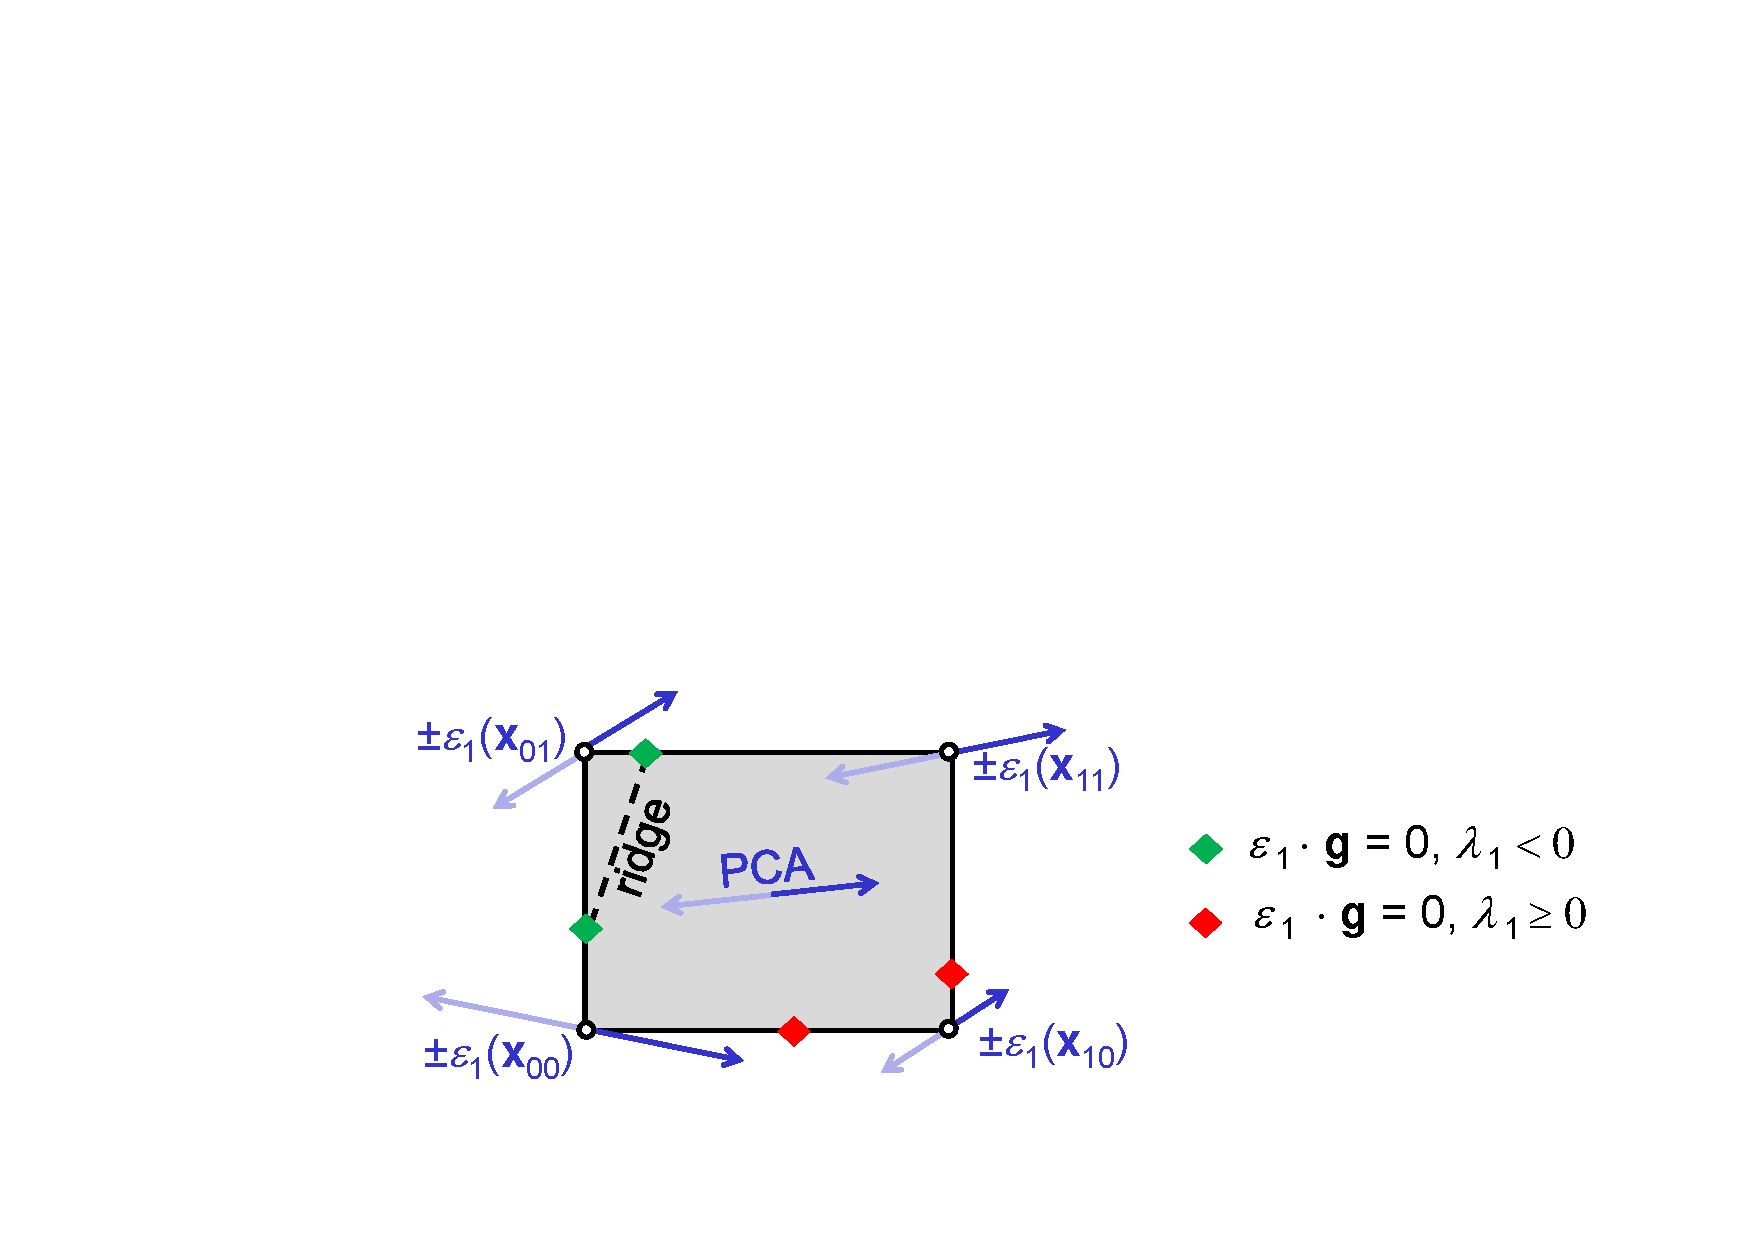
\includegraphics[width=0.6\textwidth]{img/09_ftle_ridges}
            \end{figure}

    \end{itemize}
\end{itemize}

\subsection{Lagrangian Vector Field Topology}
Alternatives for critical points:
\begin{itemize}
    \item FTLE maxima
    \item Acceleration minima [Kasten 2009]
    \item Unsteadiness minima [Fuchs 2010]
\end{itemize}

\subsubsection{Double Gyre Example}
\begin{figure}[H]
    \centering
    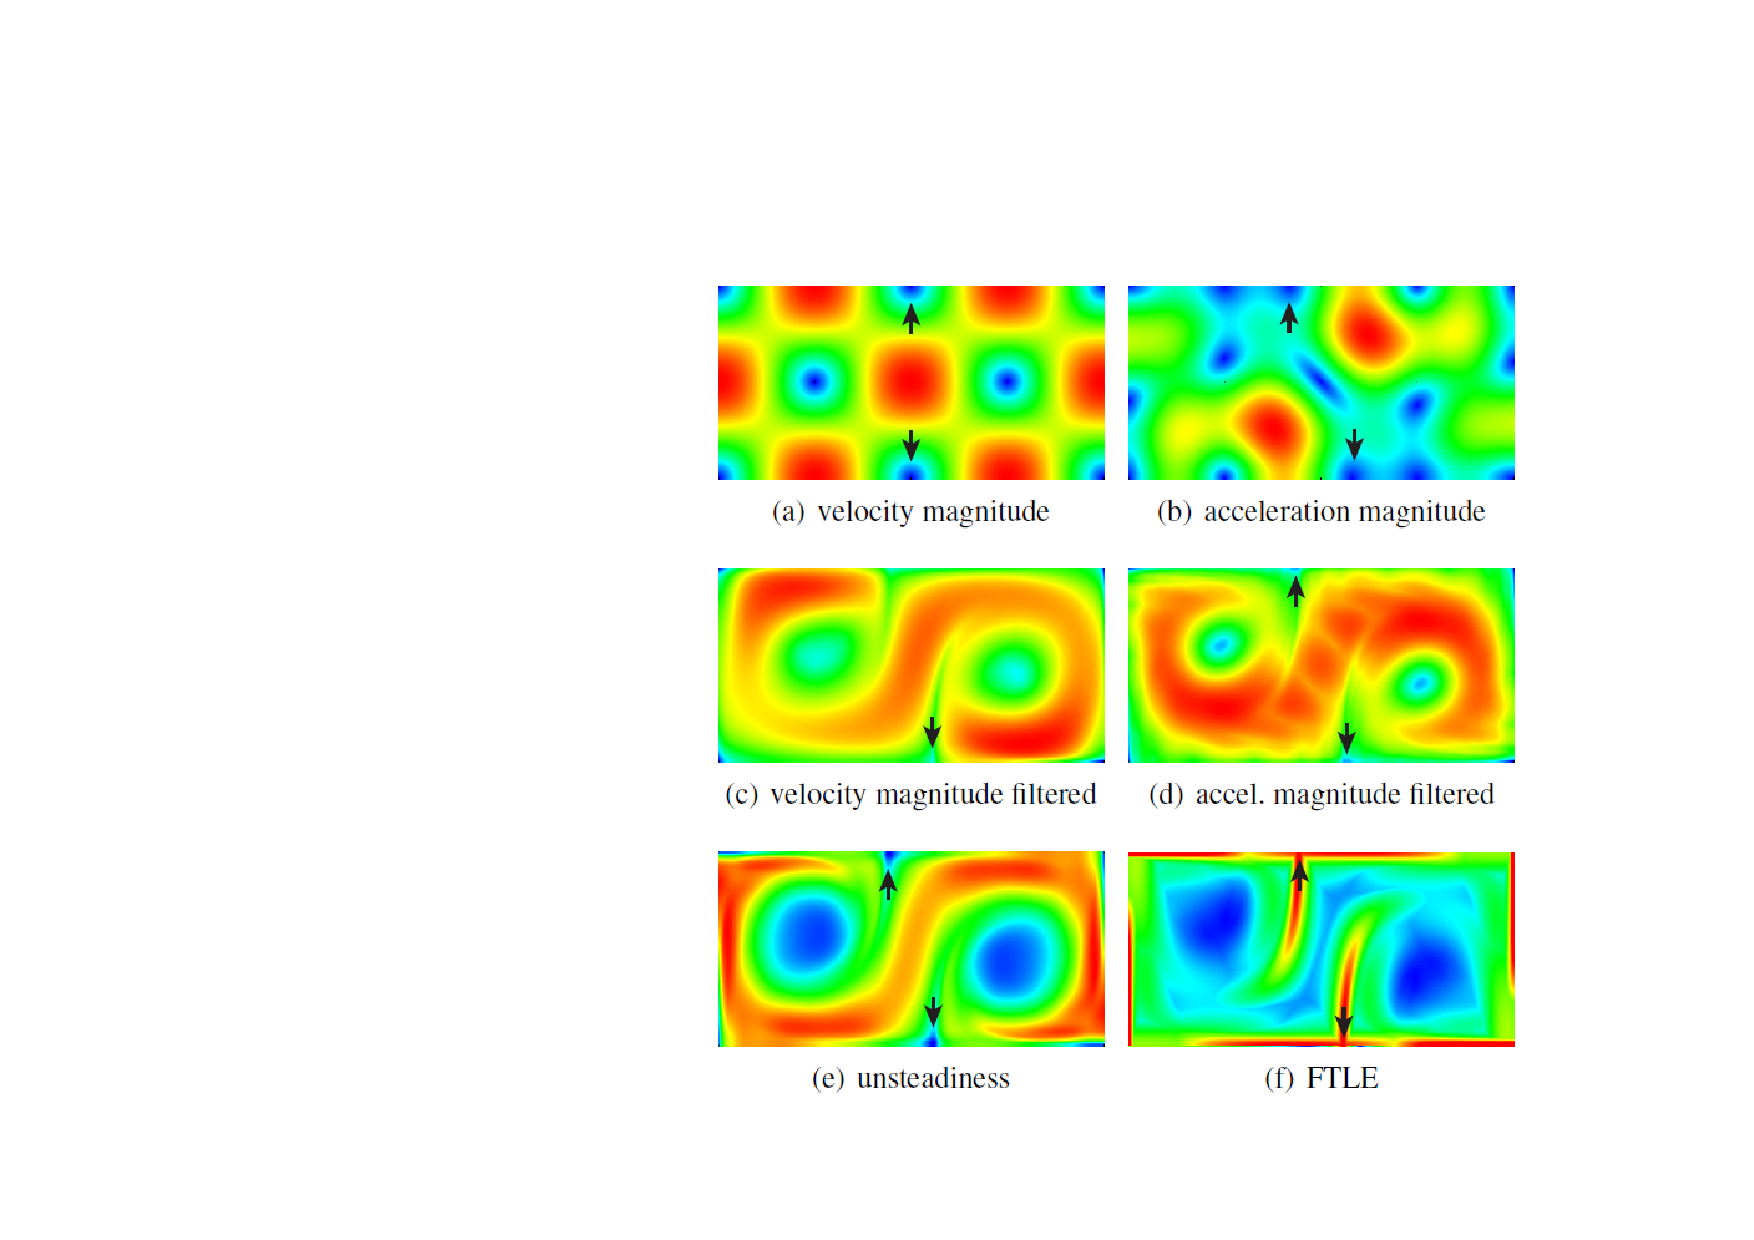
\includegraphics[width=0.6\textwidth,page=1]{img/09_lcs_examples}
\end{figure}

\subsubsection{Petri Dish Example}
\begin{figure}[H]
    \centering
    \includegraphics[width=0.55\textwidth,page=2]{img/09_lcs_examples}
\end{figure}
\newpage
\subsubsection{Vortex Street Example}
\begin{figure}[H]
    \centering
    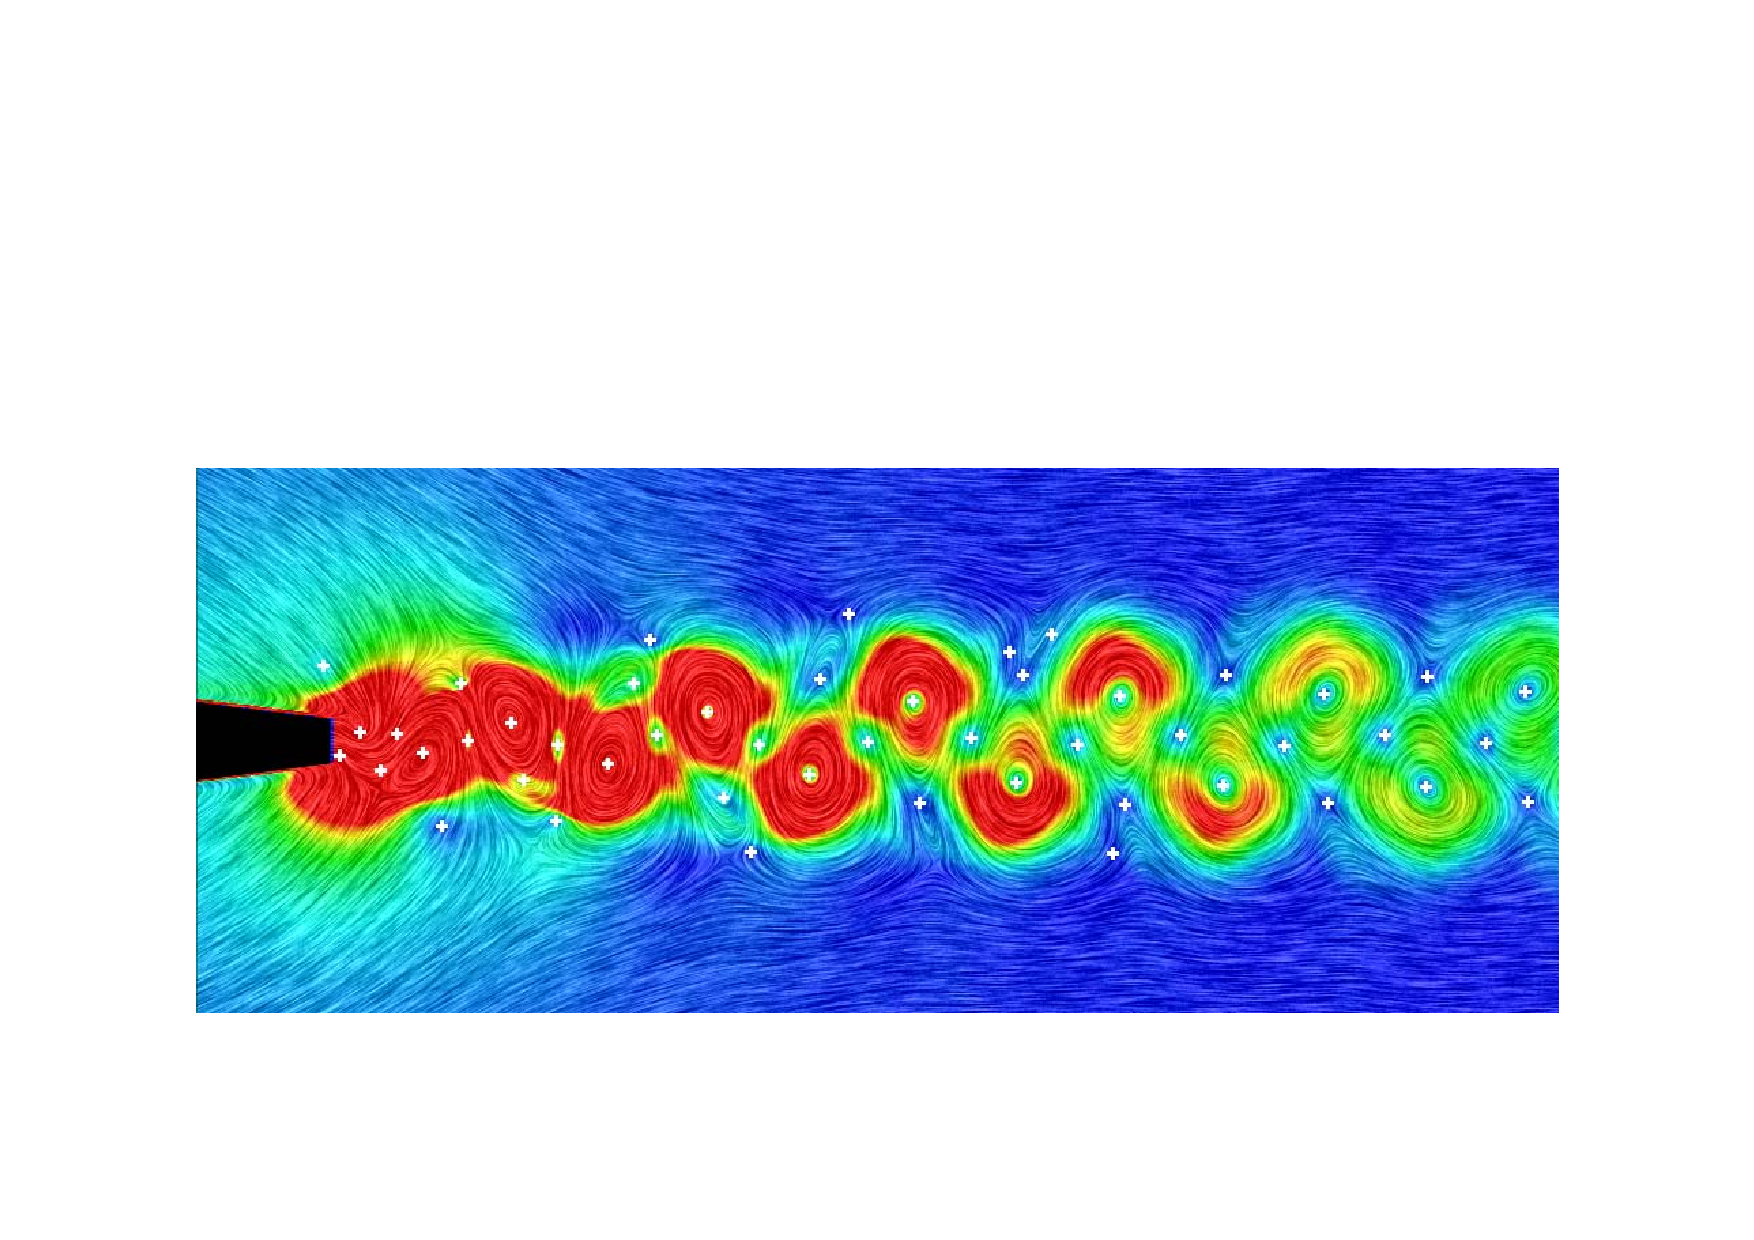
\includegraphics[width=0.55\textwidth,page=1]{img/09_vortex_street}
    \caption{Acceleration minima, temporally filterted}
\end{figure}
\begin{figure}[H]
    \centering
    \includegraphics[width=0.55\textwidth,page=2]{img/09_vortex_street}
    \caption{Velocity minima, temporally filterted}
\end{figure}
\begin{figure}[H]
    \centering
    \includegraphics[width=0.55\textwidth,page=3]{img/09_vortex_street}
    \caption{Unsteadyness minima, temporally filterted}
\end{figure}
\begin{figure}[H]
    \centering
    \includegraphics[width=0.55\textwidth,page=4]{img/09_vortex_street}
    \caption{FTLE maxima}
\end{figure}
\paragraph{Comparison} $\ $
\begin{figure}[H]
\centering
\begin{tabular}{r|ccc}
 &{Double Gyre}&{Petri Dish}&{Vortex Street}\\ \hline
 {FTLE max} & (+) & + & -\\
 {Acceleration min} & + & - & +\\
 {Unsteadiness min} & + & + & (+)
\end{tabular}

\end{figure}
























